%FROMHERE
\documentclass[12pt]{report}
\usepackage{bm}
\usepackage[a4paper,bindingoffset=25mm,%
            left=0mm,right=15mm,top=15mm,bottom=15mm,%
            footskip=5mm]{geometry}

%\usepackage{geometry}


\usepackage{relsize}
%\usepackage[Lenny]{fncychap}
\usepackage{verbatim}
\usepackage{algorithm}
\usepackage{algpseudocode}
\usepackage{listings}
\usepackage{etoolbox}

\usepackage{empheq}
\usepackage{longtable}
\geometry{
	a4paper,
	left = 25.5mm,
	top = 0mm,
	bottom = 25.5mm,
}
\usepackage{amsmath, amsthm, amssymb}
%\usepackage{nomencl}HERE
\usepackage{amsmath}
\usepackage{amsmath, amsthm, amssymb}
\usepackage{graphicx}
\usepackage{epstopdf}
%\usepackage{tabularx}
%\usepackage{breqn} 
\usepackage{caption}
\usepackage{float}
\usepackage{graphicx}
\usepackage{amsmath}
\usepackage{latexsym}
\usepackage{graphicx}
\usepackage{bm}
\usepackage{amssymb}
\usepackage{array}
\usepackage{setspace}
\usepackage{fancyhdr}
%\usepackage{citesort}
\usepackage{epstopdf}
\usepackage{xcolor}
%HERE
\usepackage{epstopdf}
\usepackage{caption}
\usepackage{float}
\usepackage{latexsym}
\usepackage{array}
\usepackage{acronym}
\usepackage{setspace}
\usepackage{fancyhdr}
\usepackage{xcolor}
\usepackage{multicol}
\usepackage{lipsum}
\usepackage{verbatim}
\usepackage{layaureo}
\usepackage{chngpage}
\usepackage{amsfonts}
\usepackage{makeidx}
\usepackage{slashbox}
\makeindex
\usepackage{enumerate}
\usepackage{calligra}
\usepackage[font={footnotesize}]{caption}
\usepackage[scr=boondoxo,
scrscaled=1.15,]{mathalfa}
\usepackage{multirow}
\usepackage{cite}
\usepackage{graphicx}
\usepackage{epstopdf}
\usepackage{url}
\usepackage[bookmarks, colorlinks=false, pdfborder={0 0 0}, pdftitle={<pdf title here>}, pdfauthor={<author's name here>}, pdfsubject={<subject here>}, pdfkeywords={<keywords here>}]{hyperref} 

%TOHERE

%\usepackage[style=ieee]{cite}
%\usepackage{cite}
%\documentclass{article}
\usepackage[utf8]{inputenc}
\usepackage[english]{babel}
%\usepackage[square,numbers]{natbib}
%\bibliographystyle{IEEEtranN}

\usepackage{setspace}
\onehalfspacing %doublespace %

\usepackage{amssymb,amsmath,amsthm}

\usepackage{cite}

\setlength{\intextsep}{1ex}

%\usepackage[dvips]{graphicx}
\usepackage{graphicx}
\include{epstopdf}
\renewcommand{\qedsymbol}{\rule{0.4em}{0.4em}}
\usepackage{tabularx}


\usepackage{lipsum}  
%\usepackage{cite}

\usepackage{float}
\setlength{\intextsep}{1ex}
\usepackage[shortlabels]{enumitem}
\usepackage{multirow}
\usepackage[font={small}]{caption}
\usepackage{nameref}

\usepackage[justification=centering]{caption}
\usepackage{caption,subcaption}
\usepackage[toc,page]{appendix}



\setlength{\parskip}{10pt}
\setlength{\parindent}{0pt}

\renewcommand{\bibname}{References}


\setlength\parindent{0pt}
\setlength{\unitlength}{1cm} 

%\documentclass{article}
\begin{document}

\begin{titlepage}
\centering

\begin{figure}[H]
\centering

\includegraphics[width=0.4\textwidth]{MAK_Logo2_png.png}%
\end{figure}


\textsc{}

\vspace{\stretch{0.1}}

{\huge \textsc{Design of a machine learning based system for pharmaceutical purchases}  \\}
\rule{3in}{0.4pt}

\vspace{\stretch{0.4}}

{\Large\textbf{Abraham Jerry Kakooza}	 \\}
Reg No.: 16/U/327\\ \vspace{2cm}
{\large \textbf{Department of Electrical and Computer Engineering} \\
School of Engineering \\
College of Engineering, Design, Art and Technology}



\vspace{\stretch{0.3}}

{
Supervisor: \textbf{Dr Andrew Katumba}    \\
Co-supervisor: \textbf{Prof. Eng. Dr. Peter Lating, iLabs Principal Investigator} }

\vspace*{\stretch{0.2}}

% Add date in desired format
December 7, 2020


\vspace*{\stretch{0.2}}
% Add the statement of what the report represents
{
A Report submitted in partial fulfillment of the requirements for the \\ \textbf{ Degree of Bachelor of Science in Telecommunications Engineering} \\ at Makerere University. }


\end{titlepage}



%\maketitle
				
%\beforeabstract %\input{abstract} 

\pagenumbering{roman}

\section*{Declaration}

\textbf{ABRAHAM KAKOOZA JERRY}

I declare that this research was completed with support from Soteria Pharmacy in Luweero District for the period from 1st August 2019 to 4th December 2020.

\emph{Academic Integrity Pledge:}

\emph{
  I have abided by the Makerere University academic integrity policy on this
assignment.
}
I also confirm that this report is only prepared for my academic requirement, not for any other
purpose.


\emph{Signature} \hspace{0.5cm} \makebox[1.5in]{\hrulefill} \hspace{0.5cm} \emph{Date} \hspace{0.5cm} \makebox[1.5in]{\hrulefill}

\newpage


\section*{Approval}

\vspace{2cm}
\begin{center}
  This report has been submitted with approval and under the supervision of the following
  supervisors:\\
  
  Main Supervisor\\
  Lecturer\\
  Department of Electrical and Computer Engineering,\\
  Makerere University\\

  \emph{Dr.Andrew Katumba} \hspace{0.5cm} \makebox[1.5in]{\hrulefill} \hspace{0.5cm} \emph{Date} \hspace{0.5cm} \makebox[1.5in]{\hrulefill}

 
  Co-Supervisor\\
  Lecturer\\
  Department of Electrical and Computer Engineering,\\
  Makerere University\\
  \emph{Prof.Peter Lating} \hspace{0.5cm} \makebox[1.5in]{\hrulefill} \hspace{0.5cm} \emph{Date} \hspace{0.5cm} \makebox[1.5in]{\hrulefill}


\end{center}




\newpage


\section*{Dedication}

\vspace{2cm}
\begin{center}
I , Kakooza Abraham Jerry , dedicate this to my parents who have been there for me in this entire study period both emotionally and financially, my supervisor Dr. Andrew Katumba, my mentors Tibabwetiza Joel, my partner Kevin Upyem, and lastly the entire ilabs team Mark Phillip and Ronald Ogwang .
\end{center}



\newpage

\section*{Acknowledgments}
I would like to thank God for enabling me to complete my Final Year Project successfully. I also extend my gratitude ti the ilabs at Mak Project for the opportunity to work with them which has given me a wealth of skills and experience to build my engineering career.\\

I highly acknowledge my main supervisor Dr. Andrew Katumba and my co-supervisor Prof. Peter Lating for the support, guidance and knowledge provided at each step of this project.\\
I highly acknowledge my mentors David Tusubira and Tibabwetiza Joel for the guidance and support.

Lastly I would like to thank the Soteria Pharmacy community, Ms. Brenda , Ms.Lydia Ssebunya and the ilabs team Mark Phillip and Ogwang Ronnie for the collective support. 

\newpage



\section*{Abstract}


To obtain inherent laws from vast amounts of pharmaceutical sales data and to provide valuable information to pharmacy managers, this work validates different methods and approaches to perform a sales forecast. Part of the data is used to train a neural network algorithm, with backpropagation for some methods, step by step, where shallow nets face selected scenarios, with different space-time data considerations. 

\indent In each method, by using a sum of square differences, and a peak search procedure, a reasonable quality in the obtained abstract representations is pursued. First, an auto-encoder is trained to develop in its hidden layer neural data abstractions about a random-moving window. Thereafter by using the abstraction of the net plus recently captured information, a second shallow net is trained to produce its own one-day ahead estimates, using new timing and data procedures. After training, the whole stacked system’s performance is compared with the naive forecast scenario’s mean square error and if it's a better value, the method is used to produce stable daily forecasting for assorted products and periods. The system has been tested in real-time with real data.

\newpage

\tableofcontents

\newpage

\listoffigures

\newpage

\listoftables

\newpage



\section*{List of Abbreviations}

\begin{tabular}{p{3cm} l}
	ARIMA	& Auto Regression Integrated Moving Average\\
	LSTM	& Long Short Term Memory\\	
  MSE & Mean Square Error\\
  KPI & Key Performance Indicator\\
  API & Application Programming Interface\\
  GPU & Graphical Processing Unit\\
  BPTT & Back Propagation Through Time\\
  RNN & Recurrent Neural Networks\\
  CNN & Convolutional Neural Network

\end{tabular}


\newpage
\pagenumbering{arabic}


\chapter{Introduction}
This chapter gives a brief explanation of the project background, problem statement,
justification, objectives, and a summary of the methodology.

\section{Project Background}
Soteria Pharmacy is a licensed Pharmacy outlet located in Luweero District and has been in operation for 4 years now. It is directly opposite the Luweero National referal hospital and close to the main road for quick access by the residents of the area.
In March 2018, Kampala and Mbale had 1029 private pharmacies with valid operating licenses from Uganda’s MRA, of which 622 were retail (licensed to dispense small quantities to patients only), 175 were wholesale (licensed to sell in bulk to retailers only) and 232 were dual (licensed for both wholesale and retail supply).\cite{14}
One of the responsibilities of pharmacies in  Uganda is to have a minimum stock of medicines.This ensures patients can have it when prescribed.
The adoption of technological tools to help in inventory tracking by pharmacies has enabled us collect vast amounts of data but all this information has not been put to full use as it only presents reports for past occurances.

In addition, pharmacies need to get a good forecast of the medication needs due to the short term validity of many medicines and the need to control stock levels.This avoids excessive costs and loss of customers due to stock outages.\\

A good sales forecast is usually associated with striking a balance between stock costs and adequate satisfaction of customer demand.People act on the basis of forecasting models whether they are on paper or in their heads. You are better off quantifying these estimations so you can discuss them rationally as opposed to making them based on intuition.\\

To specific case of pharmacies in Uganda, the problem is of particular importance due to the short cycle life of many products and the importance of quality which is in turn strongly linked to public health.

%Before digital technology dominated the world, the forecasting process was done manually by experienced individuals in the domain. This intuition required a lot of experience and was prone to error. Such a multifaceted problem started to realize the need for automating the pharmacy sales forecasting process. Research has been carried out with statistical, machine learning, deep learning and ensemble techniques to achieve more accurate sales forecasts. \cite{Perera2019}\\

During our research study of Soteria Pharmacy procurement process with an interview of Ms.Brenda the incharge of this, we realised she uses personal judgement of current stock levels athand and the rate at which people come in to ask for a ceratin drug then determine how much more stock should be purchased.Given her difficulties in accurately predicting the future sales,this report explores the product sales forecast at the indiviual level of this Pharmacy.I made a forecast for 5 sold drugs.The forecast was based on analysis of  historical data for a period of 24 months and future results analyses of 50 days determined.ARIMA and LSTM methods were used in the sales forecast of which the best model was recommended including a conclusive way of improving our results.


People act on the basis of forecasting models whether they are on paper or in their heads. One is better off quantifying these estimations so as to discuss them rationally as opposed to making them based on intuition. For pharmaceutical distribution companies, it is essential to get good estimates of drugs, due to the short shelf life of many medicines and the need to control stock levels, to avoid excessive inventory costs while guaranteeing customer demand satisfaction, and thus decreasing the possibility of a loss of customers due to stock outages.
Stock management, transportations, and financial spends contain a high percentage of total pharmaceutical companies’ expenses. As a rule, companies pay immediately when buy medications from manufacturers, and then sales compensate these spend gradually. This gap is a danger of unplanned expenses to occur. Therefore, the majority of distributors in this industry look for modern and precise forecasting methods of future sales to decrease purchase and storage costs and to increase profit by meeting clients’ needs timely.
Common existing forecasting methods are ineffective for pharmaceutical companies because these methods require a large dataset of each medication sales. In its turn, medications are constantly replaced by analogs or refreshed to enhance pharmacological effects or reduce collateral effects.
\\




\section{Problem Statement}
Our solution is addressing the high volumes of expiring drugs before purchase in pharmacies.
We anticipate that with an insight into the future sales, you can make the right purchases which
in turn minimises the inventory expenditure to incarcerate the expired medicines. Currently
pharmacies are using intuition from domain experts to identify the amount of stock to purchase
based on their current time of work in a particular place who may not be able to process large
amounts of information to cater for promotional offer sales, decision buys from wholesalers,
rotational nature of pharmacy personnel especially in large pharmacies with like first pharmacy
or even in case of a new entrant, may find a steep start up adjustment curve from wrong
estimations.





\section{Aims and Objectives}
The main aim of the research project was to precisely predict sales of drugs and medical supplies.

The specific objectives  were:

\begin{itemize}[topsep=0pt]

\item To collect datasets of previous sales and purchases from Soteria Pharmacy.

\item To train and validate datasets with ARIMA and LSTM models.

\item To optimize the best model algorithm for accurate performance.

\item To develop  a web API for pharmacies.

\end{itemize}













\section{Contributions of the Project}

The following major contributions have been accomplished during the course of this research:

\begin{enumerate}[topsep=0pt]

\item Performed a data cleaning task, analysis and training with the various Machine learning models and came up with a graphical output.

\item Developed a robust neural network model that could accurately predict future sales for a period of 50 days using a 2 year period worth of sales and purchases information.

\item Proposed a multivariate input approach with other characteristics such as precipitational weather information and promotional sales.

\end{enumerate}






\section{Organization of the Report}

This report has 3 chapters. 

\begin{itemize}
	
	\item   Introduction
	\item   Analysis and Findings which characterizes essential concepts, an overview of the categories and description of the main methods associated with the several techniques of time series analysis.
	\item 	Conclusion presents some final considerations and future work proposals.
\end{itemize}

% Describe what each chapter discusses.















\chapter{Literature Review}
% Usually Literature Review

\section{Introduction}

% Start with an introduction



Health forecasting is a novel area of forecasting,and a valuable tool for predicting future health
events or situations such as demands for health services and healthcare needs. It facilitates
preventive medicine and health care intervention strategies, by pre-informing health service
providers to take appropriate mitigating actions to minimize risks and manage demand.


\section{Literature Review}

% Add sections and (sub)subsections as appropriate
Consequently, it is required to build an accurate forecasting model of pharmaceutical preparations sales using one of the machine learning methods taking into account constant medications refreshment and a lack of previous sales data \cite{1}.

Before digital technology dominated the world, the forecasting process was done manually by experienced individuals in the domain. This intuition required a lot of experience and was prone to error. Due to this reason, they started realizing the need for automating the pharmacy sales forecasting process. 
Thus, research and experiments were carried out with statistical, machine learning, deep learning, and ensemble techniques to achieve more accurate sales forecasts. \cite{2}
Algorithms to illustrate inherent laws in large amounts of data and to forecast future data patterns have been researched since 1920. However no breakthroughs till 1980. \cite{3}
In the deep learning world, state-of-the-art performance has gained a good reputation in fields like object recognition, \cite{4} speech recognition \cite{5}, natural language processing \cite{6},
physiological effect modeling \cite{7}, and many others. More recently papers on time-series prediction or classification with deep neural networks have been reported. \cite{8,9,10,11}
Aimed at obtaining inherent laws of historical data series in pharmaceutical sales, and forecasting the demand, controlling the inventory, reducing the costs, and improving the service level, this paper designs research on the data records from a pharmacy and presents different forecasting algorithms. The testing results provide support for the fact that these algorithms greatly improve the forecast accuracy from the naive forecasting method.

\section{Data Collection}

Data mining is the search of relationships, patterns, or models that are implied on data stored
in large databases. It can be seen as the process of exploiting large amounts of data for the
purpose of identification of consistent standards, such as rules of association or time sequences
to detect systematic relationships between variables. Uses algorithms to discover rules, identify
factors and key trends, discover hidden patterns and relationships in large databases; this
information after being interpreted, is used to support decision making organizational.

\section{Machine Learning}

\subsection{Introduction}

Machine learning is a subfield of artificial intelligence (AI). The goal of machine learning generally is to understand the structure of data and fit that data into models that can be understood and utilized by people.

Although machine learning is a field within computer science, it differs from traditional computational approaches. In traditional computing, algorithms are sets of explicitly programmed instructions used by computers to calculate or problem solve. Machine learning algorithms instead allow for computers to train on data inputs and use statistical analysis in order to output values that fall within a specific range. Because of this, machine learning facilitates computers in building models from sample data in order to automate decision-making processes based on data inputs.

Any technology user today has benefitted from machine learning. Facial recognition technology allows social media platforms to help users tag and share photos of friends. Optical character recognition (OCR) technology converts images of text into movable type. Recommendation engines, powered by machine learning, suggest what movies or television shows to watch next based on user preferences. Self-driving cars that rely on machine learning to navigate may soon be available to consumers.

Machine learning is a continuously developing field. Because of this, there are some considerations to keep in mind as you work with machine learning methodologies, or analyze the impact of machine learning processes.\cite{12}




\section{Time Series Forecasting}

\subsection{Introduction}
A time series is a sequence where a metric is recorded over regular time intervals.
Depending on the frequency, a time series can be of yearly (ex: annual budget), quarterly (ex: expenses), monthly (ex: air traffic), weekly (ex: sales qty), daily (ex: weather), hourly (ex: stocks price), minutes (ex: inbound calls in a call canter) and even seconds wise (ex: web traffic).

Forecasting is the next step where you want to predict the future values the series is going to take.

Now forecasting a time series can be broadly divided into two types.\\

If you use only the previous values of the time series to predict its future values, it is called Univariate Time Series Forecasting.\\

And if you use predictors other than the series (a.k.a exogenous variables) to forecast it is called Multi Variate Time Series Forecasting


A time series is usually modelled through a stochastic process Y(t), i.e. a sequence of random variables. In a forecasting setting we find ourselves at time t and we are interested in estimating Y(t+h), using only information available at time t.\cite{13}
Anything that is observed sequentially over time is a time series.
When forecasting time series data, the aim is to estimate how the sequence of observations will continue into the future.
Forecasting involves taking models fit on historical data and using them to predict future observations.

Descriptive models can borrow for the future (i.e. to smooth or remove noise), they only seek to best describe the data.
The skill of a time series forecasting model is determined by its performance at predicting the future. This is often at the expense of being able to explain why a specific prediction was made, confidence intervals and even better understanding the underlying causes behind the problem.

\textbf{Components of Time Series} \\
Time series analysis provides a body of techniques to better understand a dataset.

Perhaps the most useful of these is the decomposition of a time series into 4 constituent parts:

\begin{enumerate}
  \item Level. The baseline value for the series if it were a straight line.
  \item Trend. The optional and often linear increasing or decreasing behavior of the series over time.
  \item Seasonality. The optional repeating patterns or cycles of behavior over time.
  \item Noise. The optional variability in the observations that cannot be explained by the model.
All time series have a level, most have noise, and the trend and seasonality are optional.

\end{enumerate}


\subsection{ARIMA}


ARIMA, short for ‘Auto Regressive Integrated Moving Average’ is actually a class of models that ‘explains’ a given time series based on its own past values, that is, its own lags and the lagged forecast errors, so that equation can be used to forecast future values.\\

An ARIMA model is characterized by 3 terms: p, d, q

where,\\

p is the order of the Auto Regression(AR) term\\

q is the order of the Moving Average(MA) term\\

d is the number of differencing required to make the time series stationary\\


A pure Auto Regressive (AR only) model is one where Yt depends only on its own lags. That is, Yt is a function of the ‘lags of Yt’.\\

Likewise a pure Moving Average (MA only) model is one where Yt depends only on the lagged forecast errors.\\

ARIMA, short for ‘AutoRegressive Integrated Moving Average’, is a forecasting algorithm based on the idea that the information in the past values of the time series can alone be used to predict the future values.
Autoregressive models often make sense for business data. They express the fact that where you go depends partly on where you are and partly on what happens to you along the way (as expressed by the random noise component).Forecasting with an autoregressive process is done with predicted values from the estimated regression equation after going forward one unit in time.

\subsubsection{Correlation and Lag Factor}
Let’s consider an example of predicting the price of gas at any particular day, say Sunday. It’s obvious and easy to think of, that Sunday’s price will be dependent on Saturday’s price.
Now let’s consider the effect of Friday’s price on Sunday’s price.

\begin{figure}[H]%[!ht]
  \begin {center}
  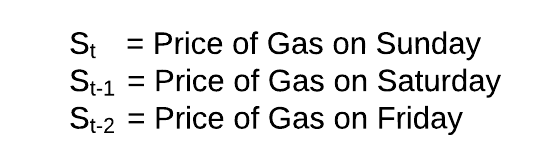
\includegraphics[width=0.95\textwidth]{images/prices.png}
  
  \label{fig:ecg}
  \end {center}
\end{figure}

As Sunday’s price is dependent on Saturday’s (2), which in-turn is dependent on Friday’s (1), there could be an indirect transitive relation between price on Friday and price on Sunday.
Aforementioned relations are visualised in the diagram below.

\begin{figure}[H]%[!ht]
  \begin {center}
  \includegraphics[width=0.95\textwidth]{images/prices_chart.png}
  \caption{AutoCorrelation}
  \label{fig:ecg}
  \end {center}
\end{figure}

Apart from these, there exists one more relation which might be difficult to imagine at first i.e. the direct effect of Friday’s price on Sunday’s price (3).
This mutual relationship between day prices here, is called correlation. If values of two variables increase (or decrease) together then they are said to have a positive correlation. If the value of one variable increases and the other decreases (or vice versa) then they have a negative correlation.

Correlation is an important concept of time series and it has 2 flavours,\\
Auto-correlation, which considers both direct and indirect effects (illustrated in the diagram above) and,\\
Partial Auto-correlation, which considers only the direct effects like in the figure below

\begin{figure}[H]%[!ht]
  \begin {center}
  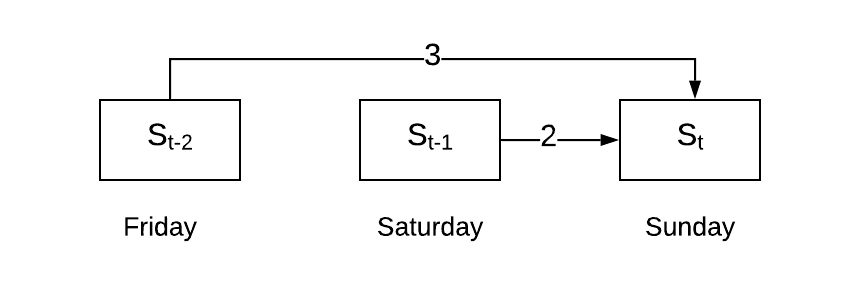
\includegraphics[width=0.95\textwidth]{images/partial_c.png}
  \caption{Partial Correlation}
  \label{fig:ecg}
  \end {center}
\end{figure}

\subsubsection{Lag Factor}
As we have considered the effect on Sunday’s price based on the price 2 days prior(i.e. Friday)… the lag factor here is 2.

\begin{figure}[H]%[!ht]
  \begin {center}
  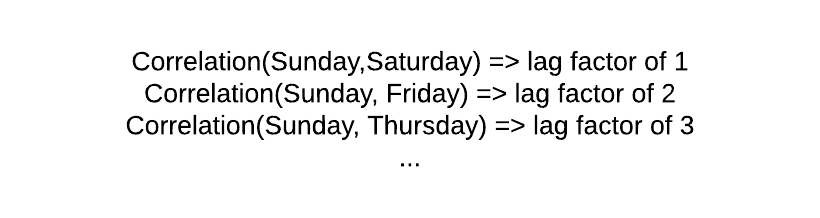
\includegraphics[width=0.95\textwidth]{images/Lag_F.png}
  \caption{Lag Factor Concept}
  \label{fig:ecg}
  \end {center}
\end{figure}

Auto-correlation and Partial Auto-correlation are important to understand before moving on to ARIMA as they are crucial for selecting the right parameters for your model. 

\subsubsection{AutoRegression(AR)}
Auto Regressive (AR) model is a specific type of regression model where, the dependent variable depends on past values of itself.
This necessarily means that the current values are correlated with values in the previous time-steps. And more specifically, the type of correlation here is partial auto-correlation.
The equation for the AR model is shown below

\begin{figure}[H]%[!ht]
  \begin {center}
  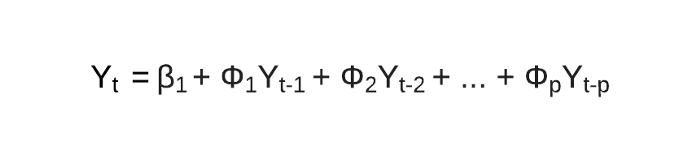
\includegraphics[width=0.95\textwidth]{images/AR_E.png}
  \caption{AR equation}
  \label{fig:ecg}
  \end {center}
\end{figure}

The respective weights of the corresponding lagged observations are decided by the correlation between… that lagged observation and the current observation. If the correlation is more, the weight corresponding to that lagged observation is high (and vice-versa).

Notice the (p) in the equation…

This (p) is called the lag order. It represents the number of prior lag observations we include in the model i.e. the number of lags which have a significant correlation with the current observation.

\subsubsection{Moving Average (MA)}
Moving Average (MA) model works by analysing how wrong you were in predicting values for the previous time-periods to make a better estimate for the current time-period.

Basically, this model factors in errors from the lagged observations. The effects of these previous(lagged) observation errors, on the current observation, depends on the auto-correlation between them. This is similar in sense as the AR model which considers the partial auto-correlations.

\begin{figure}[H]%[!ht]
  \begin {center}
  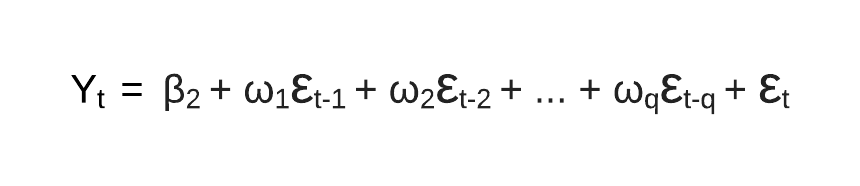
\includegraphics[width=0.95\textwidth]{images/MA_.png}
  \caption{MA equation}
  \label{fig:ecg}
  \end {center}
\end{figure}

The epsilon terms represent the errors observed at respective lags and the weights are calculated statistically depending on the correlations.
Notice the (q) in the equation…
(q) represents the size of the moving window i.e. the number of lag observation errors which have a significant impact on the current observation. Its similar to the lag order(p), but it considers errors instead of the observations themselves.

MA model supplements the AR model by taking into considerations, the errors from the previous time-periods thereby helping to get a better estimate.
When we combine the AR and MA equation we get

\begin{figure}[H]%[!ht]
  \begin {center}
  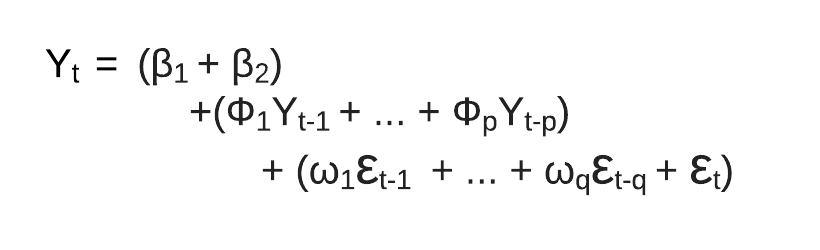
\includegraphics[width=0.95\textwidth]{images/CombinedE.png}
  \caption{Combined Equation}
  \label{fig:ecg}
  \end {center}
\end{figure}

\subsubsection{Stationary}
The models we’ve discussed so far (AR and MA) assume that the series is stationary. This is also means that “stationarity” is a necessary condition to take advantage of these models for any time series.

Basically, for a time series to be stationary, it should satisfy the following 3 conditions…\\

Mean  is constant\\
Standard Deviation  is constant\\
Seasonality doesn’t exist\\


In most cases, these conditions can be visually analysed by studying the plot against time.\\

You will came across a lot of series which are clearly not stationary.\\
Does this mean that forecasting cannot be applied in these cases ?\\
Well…this is where the sub-acronym I comes in…


\subsubsection{Integration}
Lets say, for example, you come across a series with a “non-constant” mean. Its clearly observable that the mean increases over time i.e. the series is not stationary.\\

If we could somehow eliminate this upward trend we’ll be good to go.\\
One way to do this is to consider the differences between consecutive timesteps. This is equivalent to performing a transformation of the form…


\begin{figure}[H]%[!ht]
  \begin {center}
  
\includegraphics[width=0.95\textwidth]{images/Transf.png}
  \caption{Transformation}
  \label{fig:ecg}
  \end {center}
\end{figure}

Applying this transformation we get the following trend with an observable constant mean. The standard deviation is constant as well and seasonality doesn’t exist i.e. the series is now stationary.

I stands for Integrated (though it has nothing to do with integration). It just means that, instead of predicting the time series itself we will predict the differences of the series from one time step to the next time step.
Notice that here we have taken the first order difference i.e. a single phase of differencing of consecutive terms. This is could done multiple times to make the series stationary.\cite{15}


\subsection{Forecasting with LSTM methods}
Long Short-Term Memory (LSTM) networks are a type of recurrent neural network capable of learning order dependence in sequence prediction problems.\\
Recurrent neural networks are different from traditional feed-forward neural networks.

This difference in the addition of complexity comes with the promise of new behaviors that the traditional methods cannot achieve.\\
Long-term forecasting validation has been done with three LSTM configurations: Vanilla LSTM, Stacked LSTM and Bi-directional LSTM. Relu activation function was used, optimizer was Adam and loss function was Mean Squared Error. The best results were achieved with training the model in 400 epochs. Before fitting, all data was standardized (rescaled in interval -1,1) and transformed to data for supervised problem.

\subsubsection{Recurrent Neural Networks}
Humans don’t start their thinking from scratch every second. As you read this essay, you understand each word based on your understanding of previous words. You don’t throw everything away and start thinking from scratch again. Your thoughts have persistence.

Traditional neural networks can’t do this, and it seems like a major shortcoming. For example, imagine you want to classify what kind of event is happening at every point in a movie. It’s unclear how a traditional neural network could use its reasoning about previous events in the film to inform later ones. \cite{16}

Recurrent neural networks (RNN) are a class of neural networks that are helpful in modeling sequence data. Derived from feedforward networks, RNNs exhibit similar behavior to how human brains function. Simply put: recurrent neural networks produce predictive results in sequential data that other algorithms can’t.
RNN’s and feed-forward neural networks get their names from the way they channel information.

In a feed-forward neural network, the information only moves in one direction — from the input layer, through the hidden layers, to the output layer. The information moves straight through the network and never touches a node twice.

Feed-forward neural networks have no memory of the input they receive and are bad at predicting what’s coming next. Because a feed-forward network only considers the current input, it has no notion of order in time. It simply can’t remember anything about what happened in the past except its training.

A recurrent neural network, however, is able to remember those characters because of its internal memory. It produces output, copies that output and loops it back into the network.

Simply put: recurrent neural networks add the immediate past to the present.

\begin{figure}[H]%[!ht]
  \begin {center}
  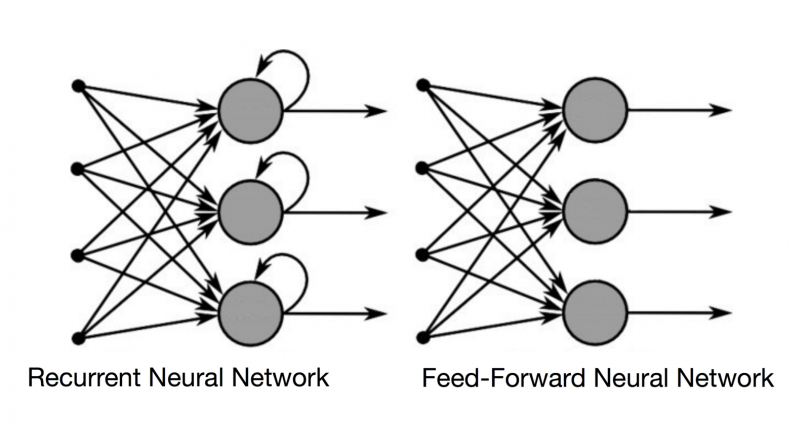
\includegraphics[width=0.95\textwidth]{images/Rnn.png}
  \caption{Feed forward RNN}
  \label{fig:ecg}
  \end {center}
\end{figure}


A feed-forward neural network assigns, like all other deep learning algorithms, a weight matrix to its inputs and then produces the output. Note that RNNs apply weights to the current and also to the previous input. Furthermore, a recurrent neural network will also tweak the weights for both through gradient descent and backpropagation through time (BPTT). 

\subsubsection{Back Propagation through time(BPTT)}

In neural networks, you basically do forward-propagation to get the output of your model and check if this output is correct or incorrect, to get the error. Backpropagation is nothing but going backwards through your neural network to find the partial derivatives of the error with respect to the weights, which enables you to subtract this value from the weights.

Those derivatives are then used by gradient descent, an algorithm that can iteratively minimize a given function. Then it adjusts the weights up or down, depending on which decreases the error. That is exactly how a neural network learns during the training process.

The image below illustrates the concept of forward propagation and backpropagation in a feed-forward neural network:

\begin{figure}[H]%[!ht]
  \begin {center}
  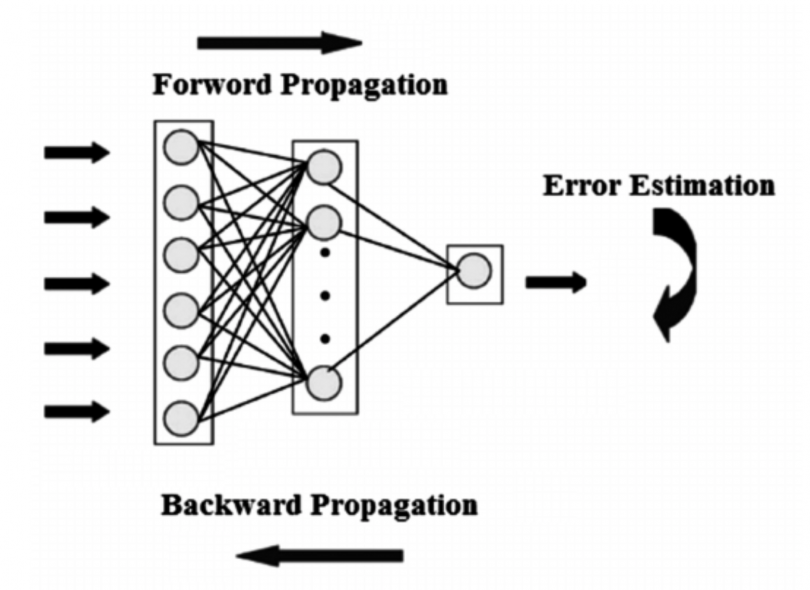
\includegraphics[width=0.95\textwidth]{images/bptt.png}
  \caption{Back Propagation Through time feed forward RNN}
  \label{fig:ecg}
  \end {center}
\end{figure}


\subsubsection{LSTM Networks}

Long Short Term Memory networks  usually just called LSTMs  are a special kind of RNN, capable of learning long term dependencies.

They were introduced by Hochreiter and Schmidhuber (1997), and were refined and popularized by many people in following work.

1.They work tremendously well on a large variety of problems, and are now widely used.

LSTMs are explicitly designed to avoid the long-term dependency problem. Remembering information for long periods of time is practically their default behavior, not something they struggle to learn.

All recurrent neural networks have the form of a chain of repeating modules of neural network. In standard RNNs, this repeating module will have a very simple structure, such as a single tanh layer.

\subsubsection{Architecture of LSTMs}
The functioning of LSTM can be visualized by understanding the functioning of a news channel’s team covering a murder story. Now, a news story is built around facts, evidence and statements of many people. Whenever a new event occurs you take either of the three steps.

Let’s say, we were assuming that the murder was done by ‘poisoning’ the victim, but the autopsy report that just came in said that the cause of death was ‘an impact on the head’. Being a part of this news team what do you do? You immediately forget the previous cause of death and all stories that were woven around this fact.

What, if an entirely new suspect is introduced into the picture. A person who had grudges with the victim and could be the murderer? You input this information into your news feed, right?

Now all these broken pieces of information cannot be served on mainstream media. So, after a certain time interval, you need to summarize this information and output the relevant things to your audience. Maybe in the form of “XYZ turns out to be the prime suspect.”.\cite{17}

A typical LSTM network is comprised of different memory blocks called cells
(the rectangles that we see in the image).  There are two states that are being transferred to the next cell; the cell state and the hidden state. The memory blocks are responsible for remembering things and manipulations to this memory is done through three major mechanisms, called gates. Each of them is being discussed below.

\subsubsection{Vanilla LSTM}
A Vanilla LSTM is an LSTM model that has a single hidden layer of LSTM units, and an output layer used to make a prediction. \cite{18}

\subsubsection{Stacked LSTM}

A Stacked LSTM architecture can be defined as an LSTM model comprised of multiple LSTM layers. An LSTM layer above provides a sequence output rather than a single value output to the LSTM layer below. Specifically, one output per input time step, rather than one output time step for all input time steps.

\subsubsection{Bidirectional LSTM}
In bidirectional RNNs, future states can also influence the present state and the past states by allowing information to flow backward. Past outputs are updated as needed depending on the new information received.

\subsection{Website Application Programming Interface(API)}
An application programming interface (API) is a computing interface that defines interactions between multiple software intermediaries. 

\subsubsection{StreamLit API}
Streamlit is an open-source app framework for Machine Learning and Data Science teams. Create beautiful data apps .\cite{19}
It is a pyhthon framework and works with Python version 3.6 - 3.8 .

\section{Summary}
% End your chapter with a short summary.

The results from the various models are to be verified using the mean square error estimator.(MSEE) The MSE is the average of the squared  differences in the values between the actual real outcome and the predicted outcome using our model. I use the MSE as a key performance indicator in order to judge if my model is performing better than those already in existance.

This project was conducted through a framework for health forecasting. The key processes
involved in developing a general health forecasting service, are illustrated below

\begin{figure}[H]%[!ht]
  \begin {center}
  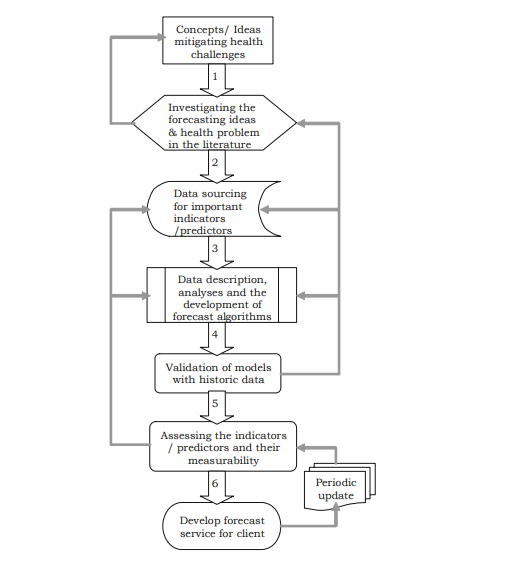
\includegraphics[width=0.95\textwidth]{images/FlowChart.png}
  \caption{The framework considered while carrying out the project}
  \label{fig:ecg}
  \end {center}
\end{figure}



























\chapter{Methodology}



\section{Materials and Methods}

% Short Introduction
We analyzed daily sales data for a period of 2 years by arranging it in a proper format to easily perform predictions with the same data file using Microsoft excel. 
It was imported into the google colab jupyter notebook by a clone from GitHub, then using pandas passed into a variable for further processing.
From box-plots, Cotrimoxazole had more outliers than the rest of the drugs which made it harder to predict future sales.
 
 We also checked for presence of seasonality and trend with a 30 day and 365 day rolling mean graph. 


\begin{figure}[H]%[!ht]
  \begin {center}
  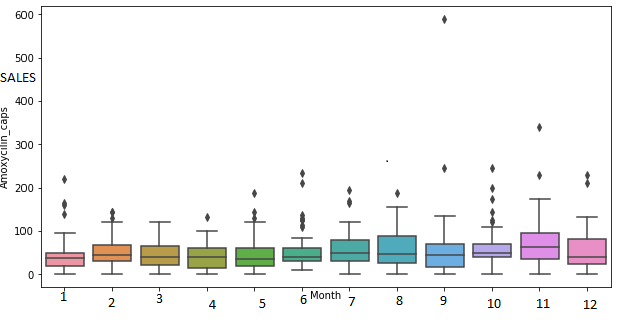
\includegraphics[width=0.85\textwidth]{images/downloadA.png}
  \caption{Box plot of the Amoxyclin Caps drug}
  \label{fig:ecg}
  \end {center}
\end{figure}

\begin{figure}[H]%[!ht]
  \begin {center}
  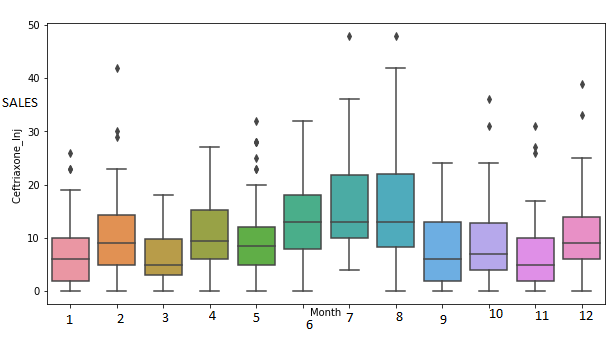
\includegraphics[width=0.85\textwidth]{images/downloadB.png}
  \caption{Box plot of Ampicloxa drug}
  \label{fig:ecg}
  \end {center}
\end{figure}

\begin{figure}[H]%[!ht]
  \begin {center}
  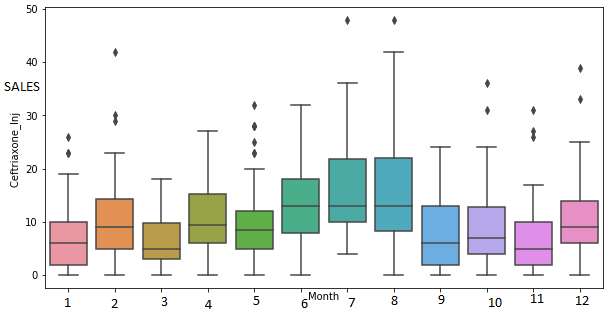
\includegraphics[width=0.85\textwidth]{images/downloadC.png}
  \caption{Box plot of Ceftriaxone Injections}
  \label{fig:ecg}
  \end {center}
\end{figure}


\begin{figure}[H]%[!ht]
  \begin {center}
  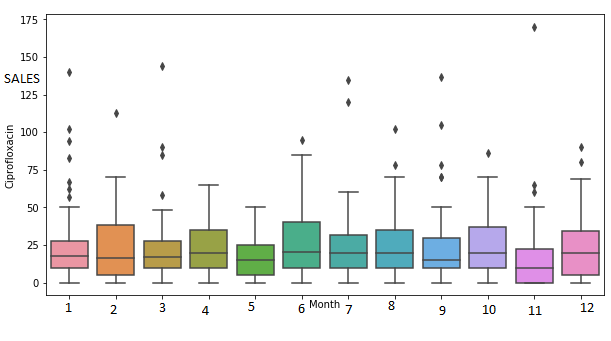
\includegraphics[width=0.85\textwidth]{images/downloadD.png}
  \caption{Box plot of Ciprofloxacin drug}
  \label{fig:ecg}
  \end {center}
\end{figure}

\begin{figure}[H]%[!ht]
  \begin {center}
  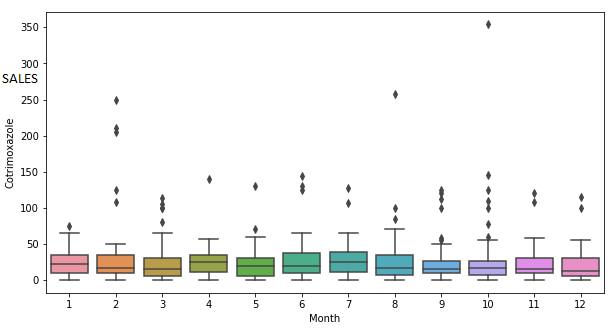
\includegraphics[width=0.85\textwidth]{images/downloadE.png}
  \caption{Box plot of Cotrimoxazole drug}
  \label{fig:ecg}
  \end {center}
\end{figure}



\begin{figure}[H]%[!ht]
  \begin {center}
  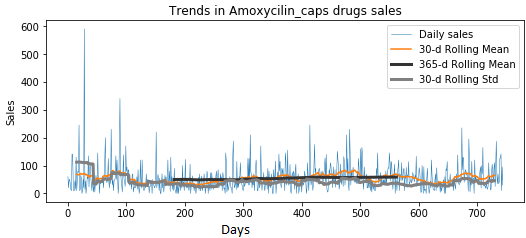
\includegraphics[width=0.95\textwidth]{images/download (10)A.png}
  \caption{Illustration plot of the trend and rolling mean for Amoxyclin Caps.}
  \label{fig:ecg}
  \end {center}
\end{figure}


\begin{figure}[H]%[!ht]
  \begin {center}
  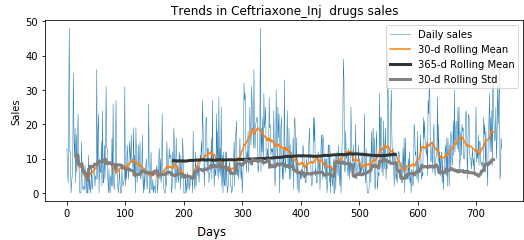
\includegraphics[width=0.95\textwidth]{images/download (10)B.png}
  \caption{Illustration plot of the trend and rolling mean for Ceftriaxone Injections.}
  \label{fig:ecg}
  \end {center}
\end{figure}

\begin{figure}[H]%[!ht]
  \begin {center}
  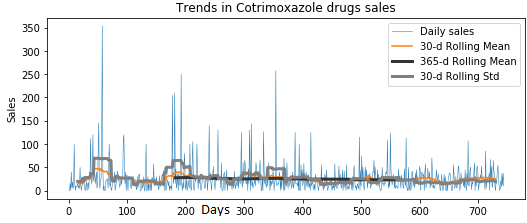
\includegraphics[width=0.95\textwidth]{images/download (10)C.png}
  \caption{Illustration plot of the trend and rolling mean for Cotrimoxazole drugs.}
  \label{fig:ecg}
  \end {center}
\end{figure}

\begin{figure}[H]%[!ht]
  \begin {center}
  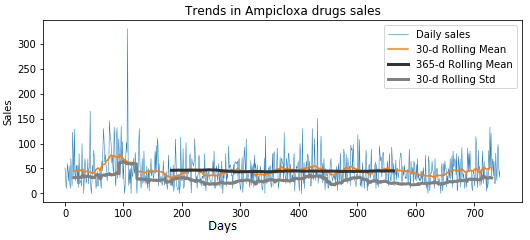
\includegraphics[width=0.95\textwidth]{images/download (12)A.png}
  \caption{Illustration plot of the trend and rolling mean for Ampicloxa drugs.}
  \label{fig:ecg}
  \end {center}
\end{figure}

\begin{figure}[H]%[!ht]
  \begin {center}
  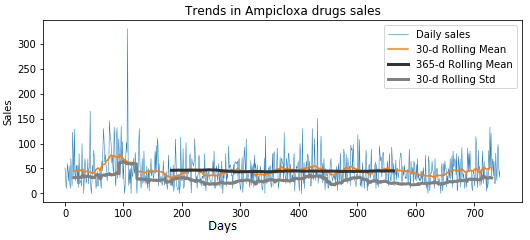
\includegraphics[width=0.95\textwidth]{images/download (12)B.png}
  \caption{Illustration plot of the trend and rolling mean for Ampicloxa drugs.}
  \label{fig:ecg}
  \end {center}
\end{figure}


\begin{figure}[H]%[!ht]
  \begin {center}
  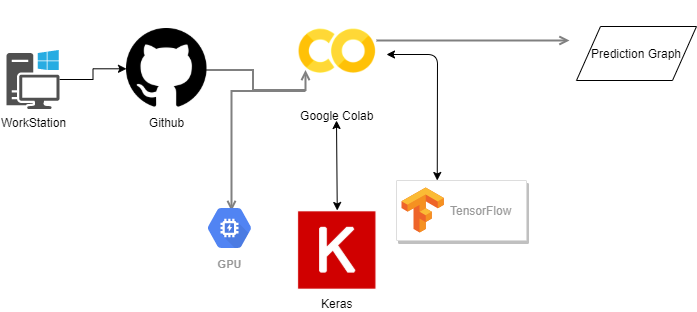
\includegraphics[width=0.75\textwidth]{images/new.png}
  \caption{Summary workflow chart.}
  \label{fig:ecg}
  \end {center}
\end{figure}

Included Components\\
\begin{enumerate}
  \item Keras: The Python Deep Learning library.
  \item Tensorflow: An open-source software library for Machine Intelligence.
  \item Github:An open-source platform to store code.
  \item Graphical Processing Unit(GPU):A processing unit for computationally intense algorithms.
\end{enumerate}


\section{Data and Results}

% Add sections and (sub)subsections as appropriate
\subsection{Naïve forecasting method}
This was the baseline method since it is what most pharmacists use during the normal day to day operation of their business for drug replenishments. Below are the results in graphical format.Our forecast values were based on the last 50 days of our 2 year period data sample.
This uses a day time shift of the previous sales to predict future sales. As a case study for soteria pharmacy in luweero district, they normally use intuition similar to this whereby the next day purchases are made basic on the previous day sales and hoping the same trend.
With our time day shift results , we modelled a naive forecasting scenario and were able to assume this as the result of what is currently being used considering most pharmacy procurement personnel use intuition.Figure 3.4 shows the plots obtained from the naive forecast scenario.

\begin{figure}[H]%[!ht]
  \begin {center}
  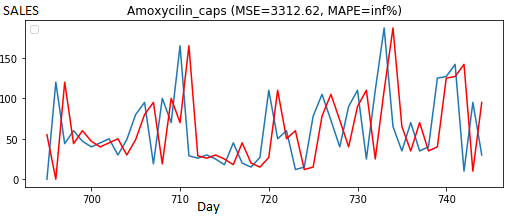
\includegraphics[width=0.75\textwidth]{images/download (13)A.png}
  \caption{Illustration plot of the Amoxycilin naïve forecasting results.}
  \label{fig:ecg}
  \end {center}
\end{figure}

\begin{figure}[H]%[!ht]
  \begin {center}
  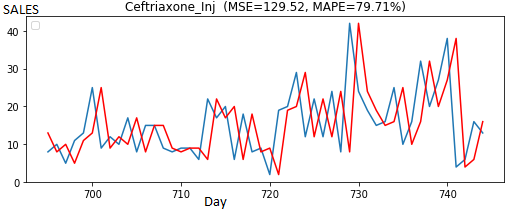
\includegraphics[width=0.75\textwidth]{images/download (13)B.png}
  \caption{Illustration plot of the Ceftriaxone naïve forecasting results.}
  \label{fig:ecg}
  \end {center}
\end{figure}

\begin{figure}[H]%[!ht]
  \begin {center}
  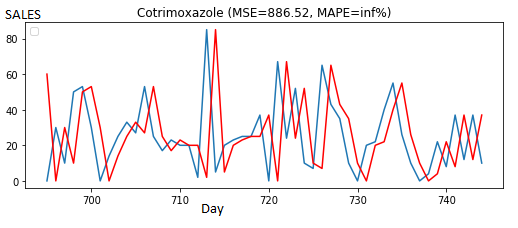
\includegraphics[width=0.75\textwidth]{images/download (13)C.png}
  \caption{Illustration plot of the Cotrimoxazole naïve forecasting results.}
  \label{fig:ecg}
  \end {center}
\end{figure}

\begin{figure}[H]%[!ht]
  \begin {center}
  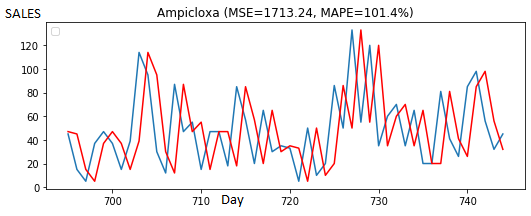
\includegraphics[width=0.75\textwidth]{images/download (14)A.png}
  \caption{Illustration plot of the Ampicloxa naïve forecasting results.}
  \label{fig:ecg}
  \end {center}
\end{figure}

\begin{figure}[H]%[!ht]
  \begin {center}
  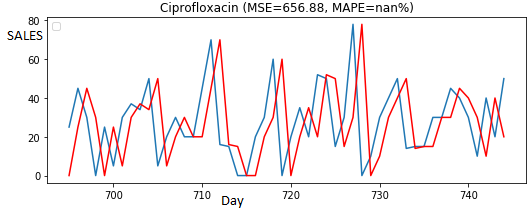
\includegraphics[width=0.75\textwidth]{images/download (14)B.png}
  \caption{Illustration plot of the Ciprofloxacin naïve forecasting results.}
  \label{fig:ecg}
  \end {center}
\end{figure}

% Add other chapters and their (sub)(sub)sections as appropriate

\subsection{ARIMA  method}


 First, method arma\_order\_select\_ic was used to determine initial p and q parameters. The method computes Akaike’s Information Criterion (AIC) for many ARIMA models and chooses the best configuration. However, AIC is not used to score accuracy of the forecasting methods in this research. Mean squared error is used instead. For that, reason, grid search optimization method was applied, where different combinations of the hyper-parameters were used to calculate MSE and then, the combination producing the least MSE was chosen as optimal. Grid search optimization for rolling forecast produced the following best combinations of the hyper-parameters:
 
Amoxyclin\_caps – Best ARIMA(1,0,0) MSE=1524.745


\subsection{Forecasting with LSTM methods}
My number of past observations tested in input sequences was 5.

I used the library Keras, which is a high-level API for neural networks and works on top of TensorFlow.

I imported the required dependencies as shown in the figure below.


\begin{figure}[H]%[!ht]
  \begin {center}
  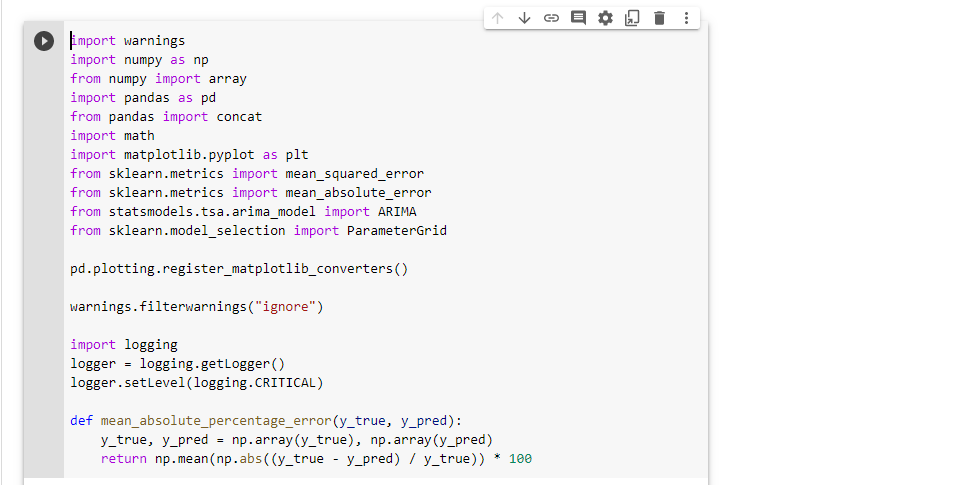
\includegraphics[width=0.95\textwidth]{images/Dependencies.PNG}
  \caption{Installing the environment Variables.}
  \label{fig:ecg}
  \end {center}
\end{figure}


\subsubsection{Vanilla LSTM}

In order to get reproducible results in forecasting with LSTM, following values are fixed: seed value, 'PYTHONHASHSEED' environment variable, Python's, numpy's and Tensorflow's built-in pseudo-random generators. A new global Tensorflow session is configured.Below are the results from the vanilla LSTM model.
This model is unidirectional in the sense that the current output is only influenced by the past states and the current input.
\begin{figure}[H]%[!ht]
  \begin {center}
  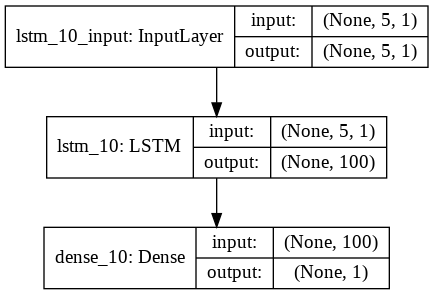
\includegraphics[width=0.75\textwidth]{dia.png}
  \caption{Vanilla LSTM model Graphical Layout.}
  \label{fig:ecg}
  \end {center}
\end{figure}

\begin{figure}[H]%[!ht]
  \begin {center}
  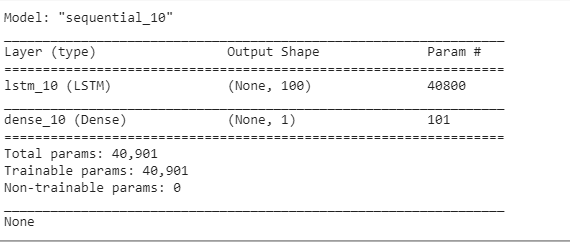
\includegraphics[width=0.75\textwidth]{VanillaSummary.png}
  \caption{Vanilla LSTM model Summary.}
  \label{fig:ecg}
  \end {center}
\end{figure}
  
  
  \begin{figure}[H]%[!ht]
    \begin {center}
    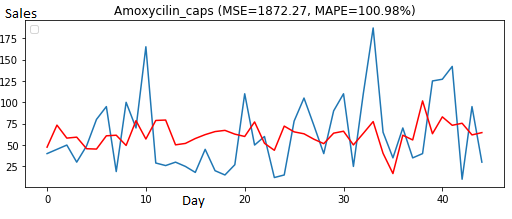
\includegraphics[width=0.75\textwidth]{images/vanilla1 (2)A.png}
    \caption{Vanilla LSTM model results for Amoxycilin Caps.}
    \label{fig:ecg}
    \end {center}
  \end{figure}
 
  \begin{figure}[H]%[!ht]
    \begin {center}
    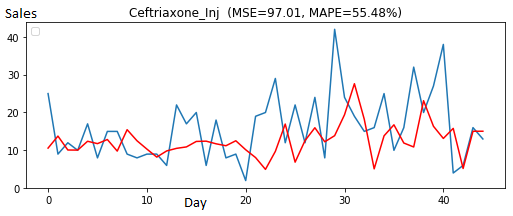
\includegraphics[width=0.75\textwidth]{images/vanilla1 (2)B.png}
    \caption{Vanilla LSTM model results for Ceftriaxone Injections.}
    \label{fig:ecg}
    \end {center}
  \end{figure}
 
  \begin{figure}[H]%[!ht]
    \begin {center}
    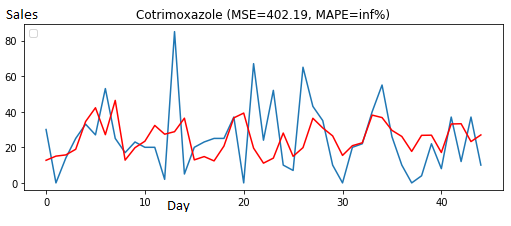
\includegraphics[width=0.75\textwidth]{images/vanilla1 (2)C.png}
    \caption{Vanilla LSTM model results for Cotrimoxazole Tabs.}
    \label{fig:ecg}
    \end {center}
  \end{figure}

  \begin{figure}[H]%[!ht]
    \begin {center}
    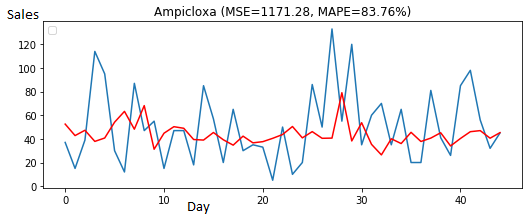
\includegraphics[width=0.75\textwidth]{images/vanilla1 (4)A.png}
    \caption{Vanilla LSTM model results for Ampicloxa Tabs.}
    \label{fig:ecg}
    \end {center}
  \end{figure}

  \begin{figure}[H]%[!ht]
    \begin {center}
    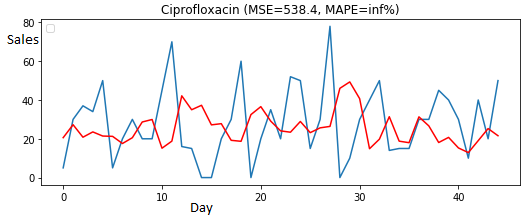
\includegraphics[width=0.75\textwidth]{images/vanilla1 (4)B.png}
    \caption{Vanilla LSTM model results for Ampicloxa Tabs.}
    \label{fig:ecg}
    \end {center}
  \end{figure}
 
 
 

  \subsubsection{Stacked LSTM method}

\begin{figure}[H]%[!ht]
\begin {center}
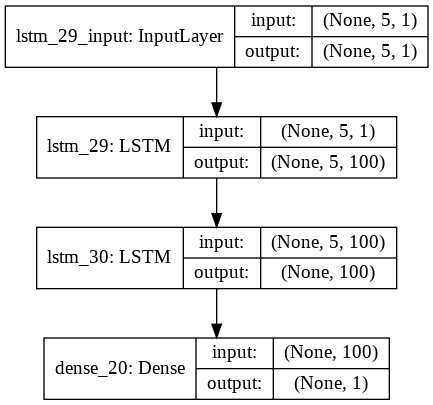
\includegraphics[width=0.75\textwidth]{StackedLstm.png}
\caption{Stacked LSTM model Graphical Layout.}
\label{fig:ecg}
\end {center}
\end{figure}

\begin{figure}[H]%[!ht]
\begin {center}
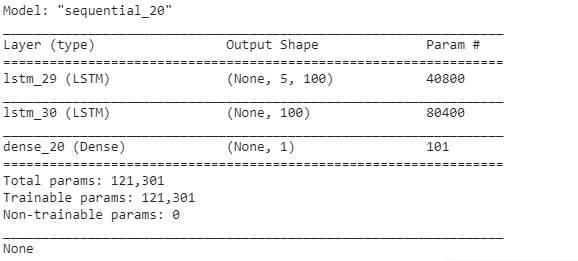
\includegraphics[width=0.75\textwidth]{StackedLstm1.png}
\caption{Stacked LSTM model Summary.}
\label{fig:ecg}
\end {center}
\end{figure}


\begin{figure}[H]%[!ht]
\begin {center}
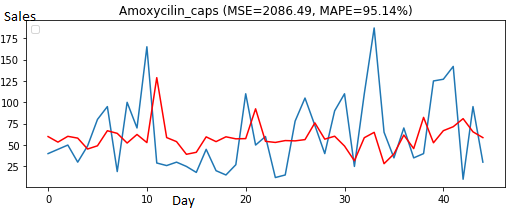
\includegraphics[width=0.75\textwidth]{images/stacked (2)A.png}
\caption{Stacked LSTM model results for Amoxycilin Tabs.}
\label{fig:ecg}
\end {center}
\end{figure}

\begin{figure}[H]%[!ht]
  \begin {center}
  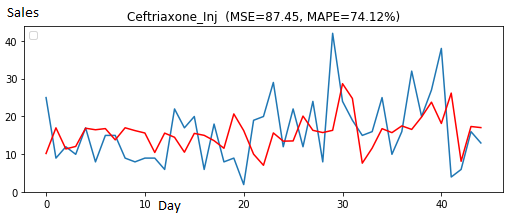
\includegraphics[width=0.75\textwidth]{images/stacked (2)B.png}
  \caption{Stacked LSTM model results for Ceftriaxone Tabs.}
  \label{fig:ecg}
  \end {center}
  \end{figure}
 
  \begin{figure}[H]%[!ht]
    \begin {center}
    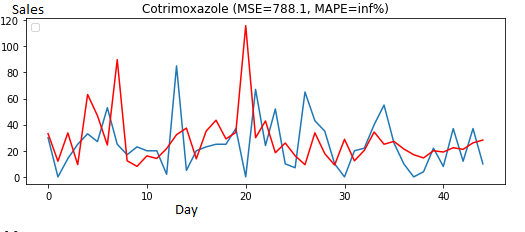
\includegraphics[width=0.75\textwidth]{images/stacked (2)C.png}
    \caption{Stacked LSTM model results for Cotrimoxazole Tabs.}
    \label{fig:ecg}
    \end {center}
    \end{figure}
    

\begin{figure}[H]%[!ht]
\begin {center}
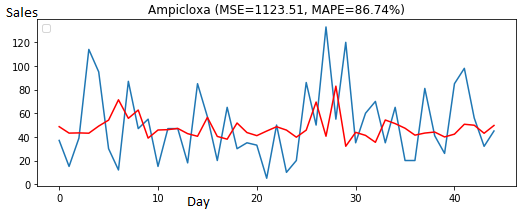
\includegraphics[width=0.75\textwidth]{images/stacked (3)A.png}
\caption{Stacked LSTM model results for Ampicloxa Tabs.}
\label{fig:ecg}
\end {center}
\end{figure}

\begin{figure}[H]%[!ht]
  \begin {center}
  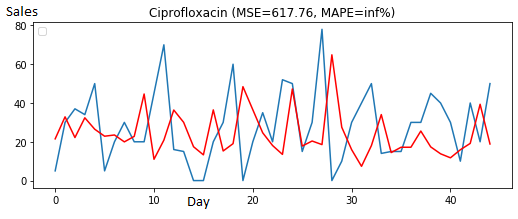
\includegraphics[width=0.75\textwidth]{images/stacked (3)B.png}
  \caption{Stacked LSTM model results for Ciprofloxacin Tabs.}
  \label{fig:ecg}
  \end {center}
\end{figure}
  

\subsubsection{Bidirectional LSTM}


\begin{figure}[H]%[!ht]
\begin {center}
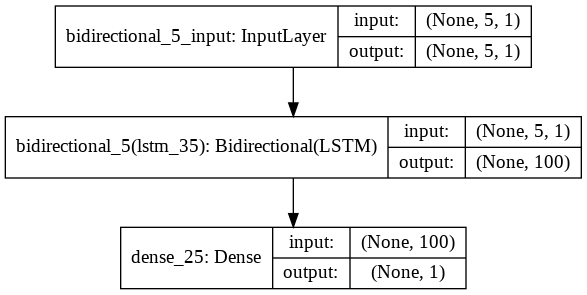
\includegraphics[width=0.75\textwidth]{Bidirectional.png}
\caption{Bidirectional LSTM model Graphical Layout.}
\label{fig:ecg}
\end {center}
\end{figure}

\begin{figure}[H]%[!ht]
\begin {center}
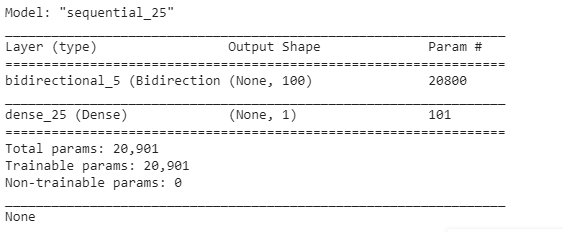
\includegraphics[width=0.75\textwidth]{Bidirectional1.png}
\caption{Bidirectional LSTM model Summary.}
\label{fig:ecg}
\end {center}
\end{figure}


\begin{figure}[H]%[!ht]
  \begin {center}
  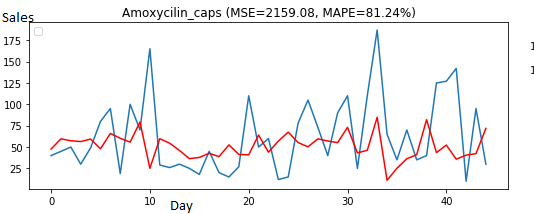
\includegraphics[width=0.75\textwidth]{images/bi (5)A.png}
  \caption{Bidirectional LSTM model results for Amoxycilin Tabs.}
  \label{fig:ecg}
  \end {center}
\end{figure}

\begin{figure}[H]%[!ht]
  \begin {center}
  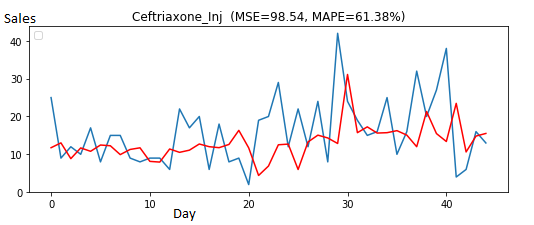
\includegraphics[width=0.75\textwidth]{images/bi (5)B.png}
  \caption{Bidirectional LSTM model results for Ceftriaxone Injections.}
  \label{fig:ecg}
  \end {center}
\end{figure}


\begin{figure}[H]%[!ht]
  \begin {center}
  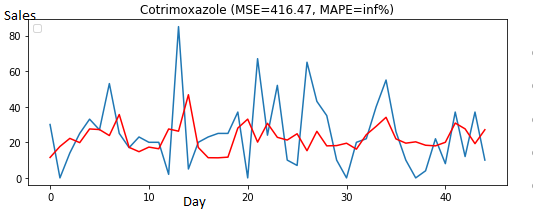
\includegraphics[width=0.75\textwidth]{images/bi (5)C.png}
  \caption{Bidirectional LSTM model results for Cotrimoxazole Tabs.}
  \label{fig:ecg}
  \end {center}
\end{figure}

\begin{figure}[H]%[!ht]
  \begin {center}
  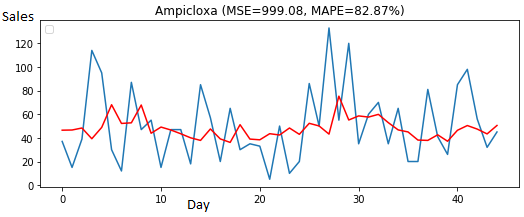
\includegraphics[width=0.75\textwidth]{images/bi (6)A.png}
  \caption{Bidirectional LSTM model results for Ampicloxa Tabs.}
  \label{fig:ecg}
  \end {center}
\end{figure}

\begin{figure}[H]%[!ht]
  \begin {center}
  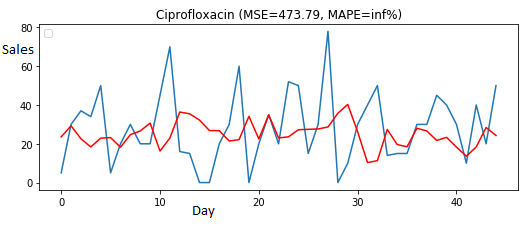
\includegraphics[width=0.75\textwidth]{images/bi (6)B.png}
  \caption{Bidirectional LSTM model results for Ciprofloxacin Tabs.}
  \label{fig:ecg}
  \end {center}
\end{figure}


\section{Web API}
I then built a web API that can be used by pharmacy managers using the streamlit python framework. One is able to select one of the various machine learning models in a drop down selection menu as shown below.
When you select the model to run , Sales data is loaded from an excel sheet and converted into the pandas data structure .This is then run and trained with the model. Results of the model are saved and used to provide an output which is the actual forecast of the model. 


\begin{figure}[H]%[!ht]
  \begin {center}
  \includegraphics[width=1\textwidth]{images/WebApp.PNG}
  \caption{Web App API.}
  \label{fig:ecg}
  \end {center}
  \end{figure}

\chapter{Discussion}

% Usually, start with a table of parameters similar to the one below, if this applies to your project.
Figure 4.1 shows that all the methods used have a less MSE than the currently used Naive forecasting methods.\\
The results from running my data with all the models are shown below.


\begin{figure}[H]%[!ht]
\begin {center}
\includegraphics[width=1\textwidth]{images/chart.png}
\caption{MSE overall results.}
\label{fig:ecg}
\end {center}
\end{figure}

However with more data of about 5 years or more, better results can be obtained for the LSTM methods .


% End with a conclusion chapter
\chapter{Conclusions and Future Works}
%\label{chap:conclusion}
This chapter contains concluding remarks of the project, that is, the conclusions, challenges met and recommendations.


\section{Conclusions}

%Conclude here
\subsection{Summary of findings}
From the work done in this project, it shows that the ARIMA model gives the lowest MSE compared to the rest of the models.
Future sales were  forecast and viewed within a Website API by the pharmacy owners in order to make informed decissions.
Data Collection was done using an inventory management system in place at Soteria Pharmacy.The various machine learning methods applied have been discussed in the report and implemented with the Mean square error as a performance metric to determine how they perform in accordance to the already existing method which is modeled as the Naive forecast in this project.


\subsection{Limitations of Study}
Among the shortcomings of our research are the reluctance of most pharmacies especially those able to provide us with the long time-span data to avail us with this information considering it is company sensitive and only known to a specific set of employees.
Also the innavailability of weather data from open platform sources hence requiring us to purchase the precipitation data from the Uganda National Metrological Association(UNMA).
It was also hard to quantize the promotional sales and factor them to have multivariate variables contribute to the input data of the Recurrent Neural Network.

\subsection{Recommendations}
We suggest that more data sets are used with a longer lifetime span of about 5 years worth data.We also suggest the incorporation of other secondary dependent features that affect the sales such as weather patterns, promotional sales, marketing elements in order to get more accurate results. 

\subsection{Acknowledgements}
I thank Dr.Andrew Katumba for the support offered at every stage of this project from day 1, he is a key component to enabling us see this idea to fruitation. We also acknowledge the management of Soteria pharmacy in Luweero district. Specifically Ms. Brenda that availed us with the required information and data plus explaining the entire workflow of the pharmacy purchasing process to us.\\

\section{Ideas for Future Work}
Incorparating a multivariate model that makes use of various input data to forecast the results such as weather data ,promotion sales data e.t.c
% Add any ideas for further work here


% You can also add a section on challenges and recommendations if you wish












%\bibliographystyle{alpha}

\medskip
%\bibliographystyle{IEEEtranN}
%\bibliography{doc}
%\bibliography{References}


\begin{thebibliography}{1}
    \bibitem{1}
    S. ~H. ~Perera, ~N. ~Jihan, ~M. ~Jayasinghe and ~Srinath "Sales forecasting using multivariate long short term memory network models,” \emph{PeerJ PrePrints,} vol. 7, pp. e27712, 2019. \hskip 1em plus 0.5em minus 0.4em \relax 

    \bibitem{2}
    Zadeh ~Khalil, ~N. ~Sepehri, ~M.~M., ~Farvaresh"Intelligent sales prediction for pharmaceutical distribution companies, A data mining based approach,” \emph{Mathematical Problems in Engineering,}  2014. \hskip 1em plus 0.5em minus 0.4em \relax 

    \bibitem{3}
    Lian-hong ~Cai, "Rough Set in Neural Network,” \emph{Computer Engineering,} Vol 27,No.5 pp65-69,2001. \hskip 1em plus 0.5em minus 0.4em \relax 

    \bibitem{4}
    Alex ~Krizhevsky, ~I ~Sutskever, and ~GE ~Hinton, "Imagenet classification with deep convolutional neural networks. Advances in Neural Information Processing Systems,” \emph{object recognition,} pages 1–9, 2012 \hskip 1em plus 0.5em minus 0.4em \relax 

    \bibitem{5}
    O ~Abdel-~Hamid and ~A ~Mohamed. "Applying convolutional neural networks concepts to hybrid NN-HMM model for speech recognition,” \emph{Acoustics, Speech, and Signal Processing,} 2012 \hskip 1em plus 0.5em minus 0.4em \relax 

    
    \bibitem{6}
    R. ~Collobert and ~Jason ~Weston. "A unified architecture for natural language processing: Deep neural networks with multitask learning,” \emph{Proceedings of the 25th international conference on Machine learning,} 2008 \hskip 1em plus 0.5em minus 0.4em \relax 

    \bibitem{7}
    HP ~Martinez. "Learning deep physiological models of affect.” \emph{Computational Intelligence Magazine,} (April):20–33, 2013. (physiological affect modelling) \hskip 1em plus 0.5em minus 0.4em \relax 

    \bibitem{8}
    Atiya, ~Amir ~F. , ~Gayar, ~Neamat ~El and ~El-~Shishiny, ~Hisham(2010) "An Empirical Comparison of Machine Learning Models for Time Series Forecasting.” \emph{Econometric Reviews,} 29: 5, 594-621  \hskip 1em plus 0.5em minus 0.4em \relax 

    \bibitem{9}
    S. ~Prasad, ~P. ~Prasad. "Deep Recurrent Neural Networks for Time Series Prediction”  \hskip 1em plus 0.5em minus 0.4em \relax 

    
    \bibitem{10}
     "DeepLearningforEvent-DrivenStockPrediction Mladen Dalto 'Deep neural networks for time series prediction with applications in ultra-short-term wind forecasting” \emph{2015 IEEE International Conference on Industrial Technology (ICIT)}   \hskip 1em plus 0.5em minus 0.4em \relax 

    
    \bibitem{11}
    XiaoDing, ~YueZhang, ~TingLiu, ~JunwenDuan, ~Mladen ~Dalto, "Deep neural networks for time series prediction with applications in ultrashort-term wind forecasting time series I” \emph{University of Zagreb, Faculty of Electrical Engineering and Computing}  \hskip 1em plus 0.5em minus 0.4em \relax 

    \bibitem{12}
     
    Lisa ~Tagliaferri"An Introduction to Machine Learning” \emph{https://www.digitalocean.com/community/tutorials/an-introduction-to-machine-learning}  \hskip 1em plus 0.5em minus 0.4em \relax 


    \bibitem{13}
     
    Davide ~Burba"An overview of time series forecasting models” \emph{https://towardsdatascience.com/an-overview-of-time-series-forecasting-models-a2fa7a358fcb}  \hskip 1em plus 0.5em minus 0.4em \relax 

    \bibitem{14}
     
    "National Drug Authority. NDA licensed outlets as at 12th March, 2018. Kampala: National Drug Authority; 2018.” \hskip 1em plus 0.5em minus 0.4em \relax 

    \bibitem{15}
     
    Accessed on December 12th 2020 "https://towardsdatascience.com/arima-simplified-b63315f27cbc” \hskip 1em plus 0.5em minus 0.4em \relax 

    \bibitem{16}
     
    Accessed on December 12th 2020 "https://colah.github.io/posts/2015-08-Understanding-LSTMs/” \hskip 1em plus 0.5em minus 0.4em \relax 

    \bibitem{17}
    Accessed on December 18th 2020, \emph{analyticsvidhya.com/blog/2017/12/fundamentals-of-deep-learning-introduction-to-lstm/}  \hskip 1em plus 0.5em minus 0.4em \relax 

    \bibitem{18}
    Accessed on December 18th 2020, \emph{https://machinelearningmastery.com/how-to-develop-lstm-models-for-time-series-forecasting/}  \hskip 1em plus 0.5em minus 0.4em \relax 

    \bibitem{19}
    Accessed on December 18th 2020, \emph{https://docs.streamlit.io/en/stable/}  \hskip 1em plus 0.5em minus 0.4em \relax 

    

\end{thebibliography}		

%% the bibliography style determines the format  in which both citations and references are printed,
%% other possible values are plain and abbrv
%%
%% If you want more control of the format of your citations you might want to take a look at
%% natbib.sty, which should be part of any standard LaTeX installation
%%
%% University regulations simply require that your citation style be consistent, so see what style
%% your supervisor recommends.

% Appendices start here



\appendix

\chapter{Appendix}


\begin{figure}[H]%[!ht]
  \begin {center}
  \includegraphics[width=1\textwidth]{images/NaiveCode.PNG}
  \caption{My Naive forecast code Base on Google Colab}
  \label{fig:ecg}
  \end {center}
\end{figure}
  
\begin{figure}[H]%[!ht]
  \begin {center}
  \includegraphics[width=1\textwidth]{images/VanillaLSTM.PNG}
  \caption{My Vanilla LSTM forecast code Base on Google Colab}
  \label{fig:ecg}
  \end {center}
\end{figure}

\begin{figure}[H]%[!ht]
  \begin {center}
  \includegraphics[width=1\textwidth]{images/StackedLSTM.PNG}
  \caption{My Stacked LSTM forecast code Base on Google Colab}
  \label{fig:ecg}
  \end {center}
\end{figure}


\begin{figure}[H]%[!ht]
  \begin {center}
  \includegraphics[width=1\textwidth]{images/MSEresults.PNG}
  \caption{Results of the machine learning forecast}
  \label{fig:ecg}
  \end {center}
\end{figure}


\end{document}
